\documentclass[11pt]{article}

% ==== PACKAGES ==== %
% \usepackage{fullpage}
\usepackage{amsmath,amssymb,amsthm}
\usepackage{epic}
\usepackage{eepic}
\usepackage{hyperref}
\usepackage{listings}
\usepackage{float}
\usepackage{graphicx}
\usepackage{fancyhdr}
\usepackage{color}
\usepackage{bbm}
\usepackage[letterpaper, margin=1in]{geometry}

% ==== MARGINS ==== %
% \pagestyle{empty}
% \setlength{\oddsidemargin}{0in}
% \setlength{\textwidth}{6.8in}
% \setlength{\textheight}{9.5in}

\pagestyle{fancy}
\fancyhf{}
\rhead{ASEN 5044}
\lhead{Homework 1}
\rfoot{Page \thepage}

\newtheorem*{solution*}{Solution}
\newtheorem{lemma}{Lemma}[section]
\newtheorem{theorem}[lemma]{Theorem}
\newtheorem{claim}[lemma]{Claim}
\newtheorem{definition}[lemma]{Definition}
\newtheorem{corollary}[lemma]{Corollary}
\lstset{moredelim=[is][\bfseries]{[*}{*]}}

% ==== DOCUMENT PROPER ==== %
\begin{document}

\thispagestyle{empty}

% --- Header Box --- %
\newlength{\boxlength}\setlength{\boxlength}{\textwidth}
\addtolength{\boxlength}{-4mm}

\begin{center}\framebox{\parbox{\boxlength}{\bf
      Statistical Estimation \hfill Homework 5\\
      ASEN 5044 Fall 2018 \hfill Due Date: October 18, 2018\\
      Name: Andrew Kramer \hfill PhD Student
}}
\end{center}

\section*{Problem 1}
A system satisfies the partial differential equation
\begin{equation*}
	\ddot{z}+10\dot{z}+100z=f(t), \quad z(0)=\dot{z}(0)=0
\end{equation*}
where $z(t)$ is the response variable (e.g. position) and $f(t)$ is a white noise forcing function with a PSD of 10 'units'.

\subsection*{part (a)}
Let $z$ and $\dot{z}$ be the state variables for this system. Write out the dynamics for this CT system in stochastic LTI form.

\subparagraph*{}
If $x=[z,\ \dot{z}]^T$, then the system in LTI form is expressed as
\begin{equation*}
	\dot{x} = \begin{bmatrix} \dot{z} \\ \ddot{z} \end{bmatrix} = \begin{bmatrix} 0 & 1 \\ -100 & -10 \end{bmatrix}\begin{bmatrix} z \\ \dot{z}\end{bmatrix} + \begin{bmatrix} 0 \\ 1 \end{bmatrix} f(t)
\end{equation*}

\subsection*{part (b)}
Suppose this process is sampled at a uniform rate beginning at time $t=0$, with $\Delta T=0.2$ seconds. Convert the CT stochastic LTI model from part (a) into DT form, and report the corresponding $F$ and $Q$ matrices.

\subparagraph*{}
\begin{equation*}
	F=\begin{bmatrix} 0.151 & 0.042 \\ -4.193 & -0.269 \end{bmatrix} \qquad Q = \begin{bmatrix} 0.004 & 0.009 \\ 0.009 & 0.376 \end{bmatrix}
\end{equation*}

\subsection*{part (c)}
Suppose the units of $z$ are in meters and $\dot{z}$ are in m/s. Provide the corresponding units of the elements of $Q$, and explain what $Q$ says physically about the elements of the DT process noise vector $w(k)$ and its effect on the DT state $x(k)$.

\subparagraph*{}
If $x_1$ is in m and $x_2$ is in m/s, then the units of $Q_{1,1}$ are in $\text{m}^2$ and $Q_{2,2}$ are in $(\text{m/s})^2$. Because $Q$ is the covariance of the multivariate white gaussian noise distribution, the diagonal elements of $Q$ represent the variances of the additive noise to the state vector and the off-diagonal elements represent their covariances.

\subsection*{part (d)}
Suppose a sensor is attached to this system, with the CT model $y(t)=z+\dot{z}\Delta T+\tilde{v}(t)$, where $\tilde{v}(t)$ is a white noise input with PSD of 3 units. Report the $H$ and $R$ matrices for the corresponding DT model; also report the units of $R$ if $z$ has units of meters.

\subparagraph*{}
\begin{equation*}
	H=[1\ \Delta T]^T
\end{equation*}
Because $y(k)$ is a scalar, the $R$ 'matrix' is simply the 1D variance of the additive white gaussian noise. This means $R=3$.

\section*{Problem 2}
Consider a battery with a completely unknown voltage ($P_0=\infty$). Two independent measurements of the voltage are taken to estimate the voltage, the first with a variance of 1 and the second with a variance of 4.

\subsection*{part (a)}
Write the weighted least squares voltage estimate in terms of the two measurements $y_1$ and $y_2$.

\subparagraph*{}
The measurement model for this system is $y(k)=Hx+\mathcal{N}(0,R)$ where $y=[y_1,\ y_2]^T$, $H=[1,\ 1]^T$, and 
\begin{equation*}
	R = \begin{bmatrix} 1 & 0 \\ 0 & 4 \end{bmatrix}
\end{equation*}
So the weighted least squares estimate of this system's state is
\begin{align*}
	\hat{x}_{LS} &= (H^TR^{-1}H)^{-1}H^TR^{-1}y \\
	&= \Bigg\{ [1\ 1] \begin{bmatrix} 1&0\\0&4 \end{bmatrix} \begin{bmatrix} 1\\1 \end{bmatrix} \Bigg\}^{-1} [1\ 1] \begin{bmatrix} 1&0\\0&4 \end{bmatrix} \begin{bmatrix} y_1 \\ y_2 \end{bmatrix} \\
	&= 1.25^{-1} [1\ 0.25]\begin{bmatrix} y_1 \\ y_2 \end{bmatrix} \\
	&= \frac{y_1 + 0.25y_2}{1.25}
\end{align*}

\subsection*{part (b)}
If weighted least squares is used to estimate the voltage, what is the variance of the voltage estimate after the first measurement? After the second measurement?

\subparagraph*{}
The covariance of the estimate is calculated as $P_e=(H^TR^{-1}H)^{-1}$. The covariance after the first measurement is simply $(1\times1^{-1}1)^{-1}=1$. The covariance after the second measurement is
\begin{equation*}
	\Bigg\{ [1\ 1] \begin{bmatrix} 1 & 0 \\ 0 & 4 \end{bmatrix} \begin{bmatrix} 1\\1 \end{bmatrix} \Bigg\}^{-1} = 0.8
\end{equation*}

\subsection*{part (c)}
If the voltage is estimated as $(y_1+y_2)/2$, what is the variance of the voltage estimate?

\subparagraph*{}
In this case $\hat{x}$ is estimated as $(H^TH)^{-1}H^Ty$. This means the estimation error $e=-(H^TH)^{-1}H^Tv$. Because of this the estimate covariance becomes
\begin{align*}
	P_e &= E(ee^T) \\
	&= E((H^TH)^{-1}H^Tv\{\dots\}^T) \\
	&= (H^TH)^{-1} H^T E(vv^T) (H^T)^T(H^TH)^{-T} \\
	&= (H^TH)^{-1} H^T R H(H^TH)^{-T} \\
	&= \frac{1}{2} \begin{bmatrix} 1 & 1 \end{bmatrix} \begin{bmatrix} 1 & 0 \\ 0 & 4 \end{bmatrix} \begin{bmatrix} 1 \\ 1 \end{bmatrix} \frac{1}{2} \\
	&= 1.25
\end{align*}

\section*{Problem 3}
The production of steel in the United States between 1946 and 1956 was 66.6, 84.9, 88.6, 78.0, 96.8, 105.2, 93.2, 111.6, 88.3, 117.0, and 115.2 million tons. Find the least squares fit to these data using the following functions. Include a plot of the original data along with the least squares curve, the rms error of the least squares fit, and a prediction for steel production in 1957.

\subsection*{part (a)}
Linear Curve Fit

\subparagraph*{}
The RMS error for the linear fit is $8.7823$ and the predicted steel production for 1957 is $118.715$ million tons. Figure \ref{p1_plot1} shows the estimated vs actual steel production for 1946 through 1956.
\begin{figure}[h!]
	\centering
	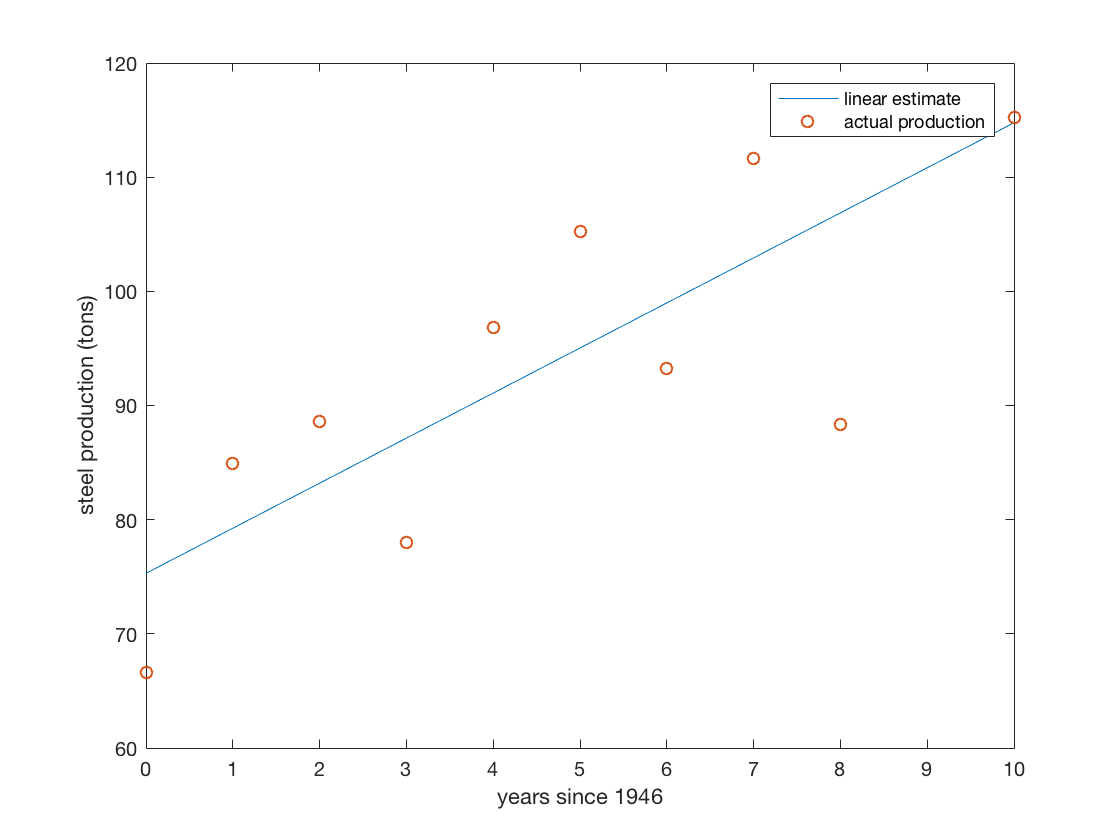
\includegraphics[width=0.8\linewidth]{p1_plot1.png}
	\caption{estimated vs actual state for linear fit}
	\label{p1_plot1}
\end{figure}

\subsection*{part (b)}
Quadratic Curve Fit

\subparagraph*{}
The RMS error for the linear fit is $8.6665$ and the predicted steel production for 1957 is $114.530$ million tons. Figure \ref{p1_plot2} shows the estimated vs actual steel production for 1946 through 1956.
\begin{figure}[h!]
	\centering
	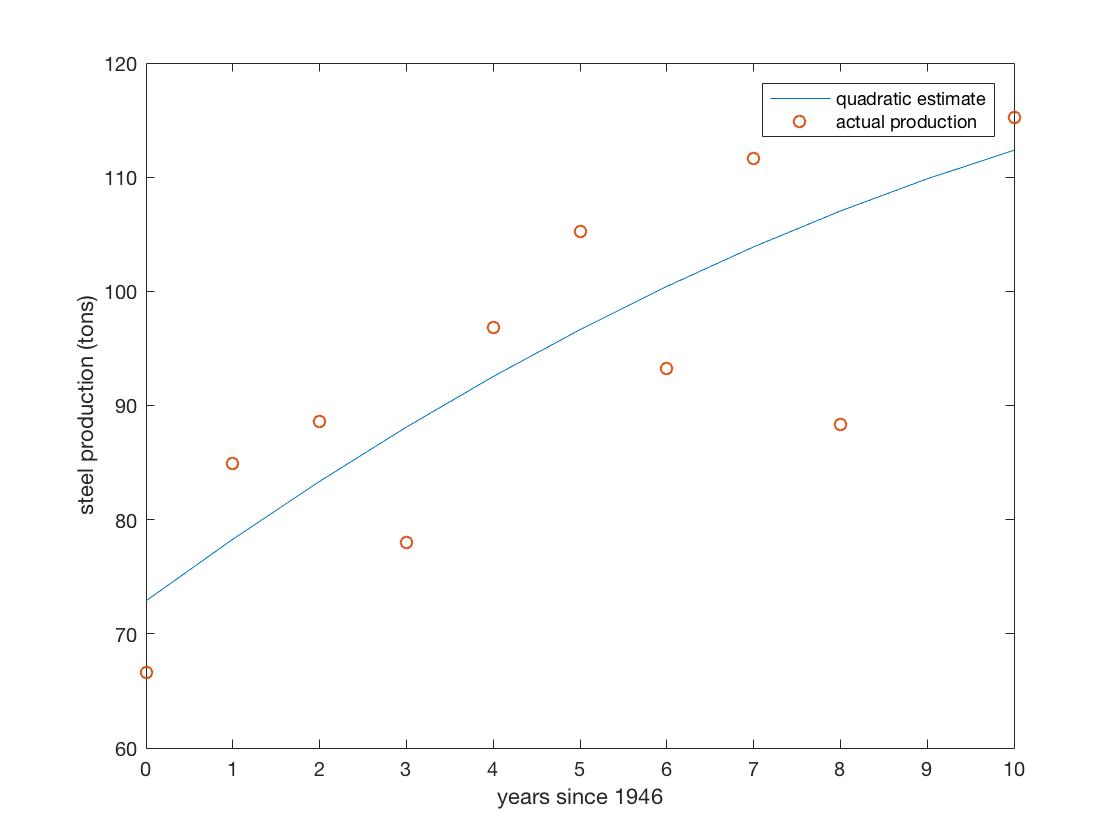
\includegraphics[width=0.8\linewidth]{p1_plot2.png}
	\caption{estimated vs actual state for quadratic fit}
	\label{p1_plot2}
\end{figure}

\subsection*{part (c)}
Cubic Curve Fit

\subparagraph*{}
The RMS error for the linear fit is $8.2889$ and the predicted steel production for 1957 is $126.188$ million tons. Figure \ref{p1_plot3} shows the estimated vs actual steel production for 1946 through 1956.
\begin{figure}[h!]
	\centering
	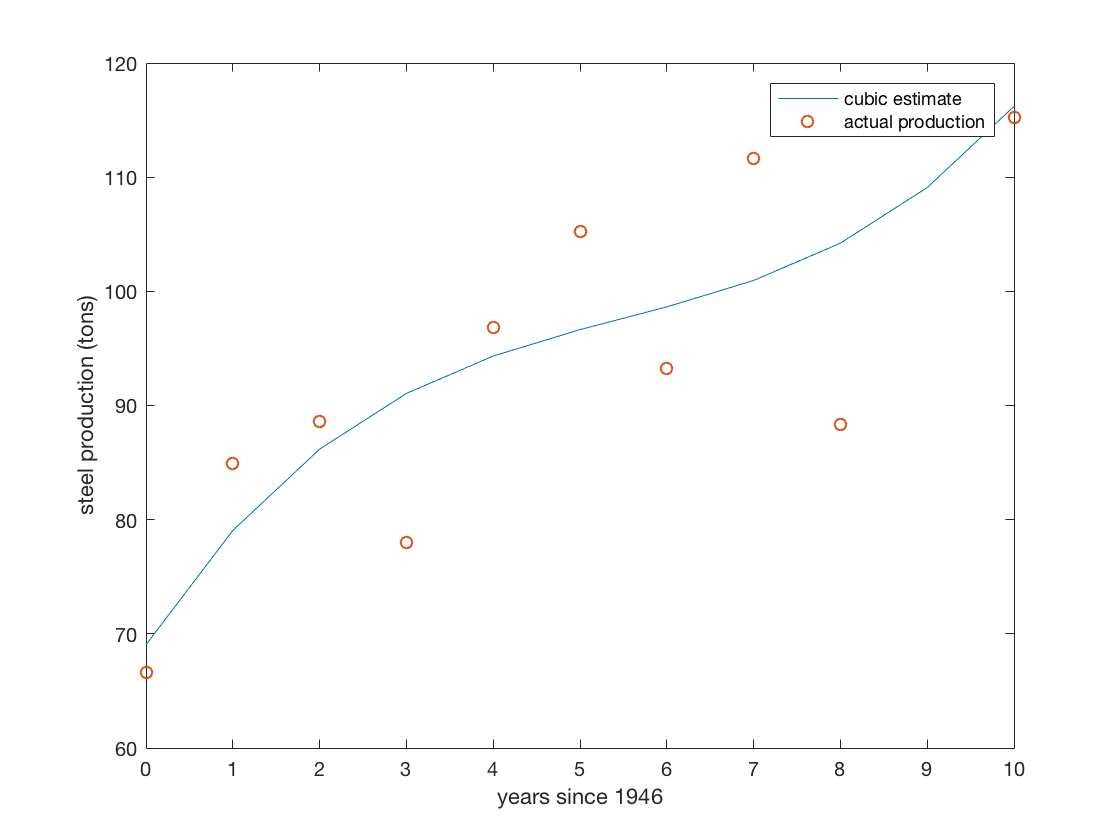
\includegraphics[width=0.8\linewidth]{p1_plot3.png}
	\caption{estimated vs actual state for cubic fit}
	\label{p1_plot3}
\end{figure}

\subsection*{part (d)}
Quartic Curve Fit

\subparagraph*{}
The RMS error for the linear fit is $8.2816$ and the predicted steel production for 1957 is $128.861$ million tons. Figure \ref{p1_plot4} shows the estimated vs actual steel production for 1946 through 1956.
\begin{figure}[h!]
	\centering
	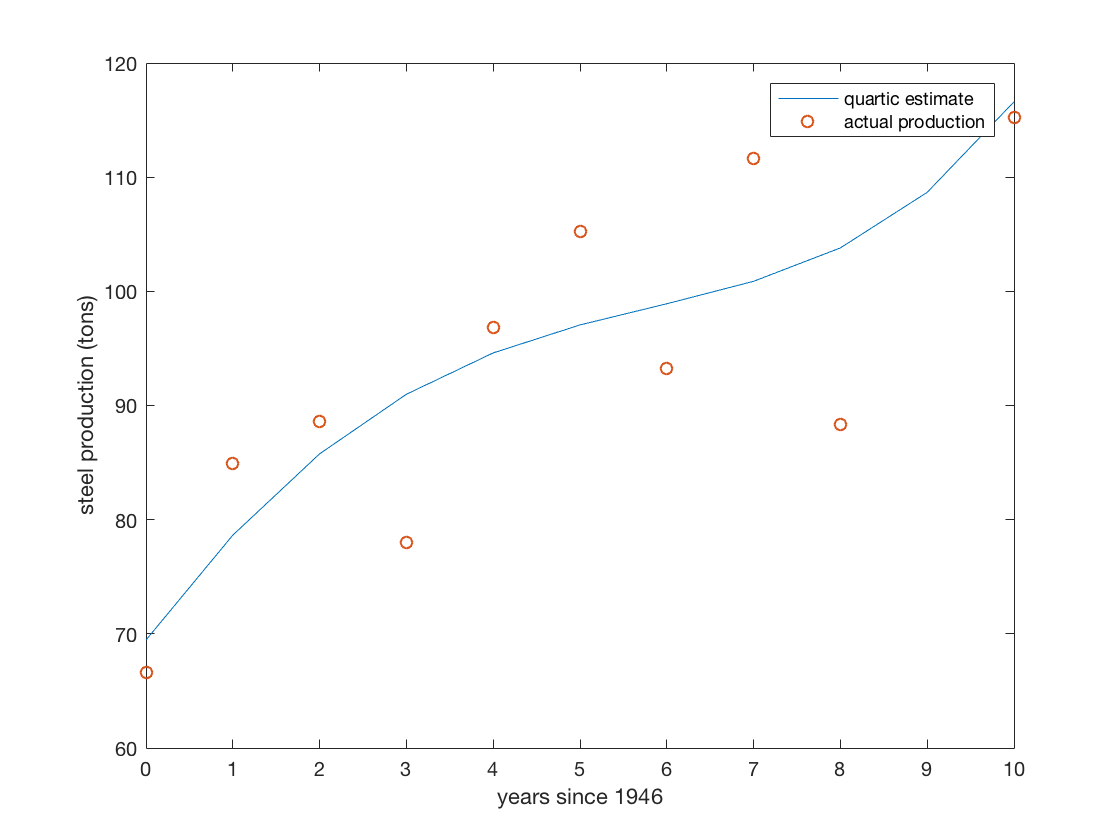
\includegraphics[width=0.8\linewidth]{p1_plot4.png}
	\caption{estimated vs actual state for cubic fit}
	\label{p1_plot4}
\end{figure}

\section*{Problem 4}
Consider the 3D static robot GPS localization problem defined in Lecture 19. Suppose the AWGN sensor error covariance matrix is given by 
\begin{equation*}
	R=\begin{bmatrix} 8 & 5.15 & 6.5 \\ 5.15 & 5 & -4.07 \\ 6.5 & -4.07 & 50 \end{bmatrix}
\end{equation*}

\subsection*{part (a)}
Suppose the true robot position is known to be at $\xi_0=\eta_0=z_0=1\text{m}$. Simulate $T=100$ measurements for the robot at this location and provide three separate 2D scatter plots of the resulting simulated noisy $y$ data: one showing all $y_k(1)$ vs $y_k(2)$, another showing all $y_k(1)$ vs $y_k(3)$, and another showing all $y_k(2)$ vs $y_k(3)$. Use the same scales on both axes for all of the plots.

\subsection*{part (b)}
Compute the sample covariance matrix for the simulated measurement vectors from part (a). How does the estimated covariance compare to $R$?

\subsection*{part (c)}
Use the simulated data from part (a) to estimate the robot's 3D position via batch weighted least squares using the first 3 samples, then the first 10 samples, and finally using all 100 samples. Report the \textbf{estimation error covariance} matrix in all 3 cases (be sure to provide units). How accurate are these estimates compared to the ground truth?

\subsection*{part (d)}
Using the data log of $y(k)$ vectors over $T'=30$ time steps in the \texttt{hw6problem5data.csv} file provided on D2L, estimate the robot's position using batch weighted least squares and report the estimated error covariance matrix (be sure to provide units).

\subsection*{part (e)}
Repeat (d) using batch unweighted least squares. Compare the final result and its covariance to the results from part (d).

\subsection*{part (f)}
Repeat (d) using recursive weighted least squares and report the results by showing a separate plot for each of the estimated states (using solid lines) and their associated $\pm2\sigma$ error bounds (using dashed lines) evolving vs time step $k$. In other words, plot how the state estimate and error bounds evolve as each new measurement vector $y(k)$ comes in for $k=1$ to $T'$ and be sure to provide units.

\end{document}
